\begin{figure}
    \centering
    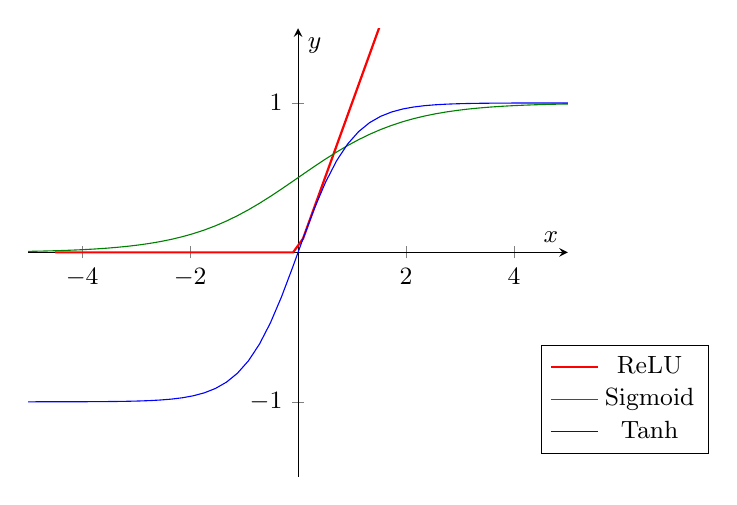
\begin{tikzpicture}
        \begin{axis}[
            axis lines = middle,
            xlabel = \(x\),
            ylabel = \(y\),
            xmin=-5.0,
            xmax=5.0,
            ymin=-1.5, 
            ymax=1.5,
            legend entries={ReLU,tanh,sigmoid},
            legend style={at={(0.95,0.05)},anchor=south west},
            %legend image post style={sharp plot,draw=red},
            cycle list name=color list,
            font=\small,
        ]
        % ReLU
        \addplot[color = red, thick, domain=-4.5:4.5, samples = 50] {max(0,x)};
        \addlegendentry{ReLU}
        % Sigmoid
        \addplot[color = green!50!black, samples=50] {1/(1+exp(-x))};
        \addlegendentry{Sigmoid}
    
        % tanh
        \addplot[color = blue, samples=50] {tanh(x)};
        \addlegendentry{Tanh}
        \end{axis}
    \end{tikzpicture}
    \caption{Activation Functions (ReLU, Sigmoid, Tanh) - Activation functions determine the output of a neuron in a neural network, and ReLU, Sigmoid, and Tanh are some commonly used activation functions that enable non-linear transformations of input data.}
    \label{fig:Activation Functions}
\end{figure}
